\section{Primary Security and Utility Results}
\subsection{Retrieval exposure and generated disclosure}
Table~\ref{tab:main} shows the central security result. Global retrieval exposes unauthorized context in every one of 1,750 unauthorized prompt-only requests. Both secured architectures reduce observed \ucer{} to 0/1,750. The Wilson 95\% upper bound for 0/1,750 is 0.219\%, so this result is evidence of strong performance under the modeled ACL, not proof that real-world risk is zero.

\begin{table}[t]
\caption{Primary security and utility outcomes.}
\label{tab:main}
\centering
\footnotesize
\begin{tabular}{lccc}
\toprule
Metric & Prompt-only & Pre-ACL & Risk-aware \\
\midrule
\ucer{} (unauth.) & 1750/1750 & 0/1750 & 0/1750 \\
\udr{} canary & 5/1750 & 0/1750 & 0/1750 \\
\arsr{} ($k=2$) & 790/1000 & 640/1000 & 705/1000 \\
\frr{} & 0/1000 & 0/1000 & 0/1000 \\
\arsr{} (controlled $k=1$) & 895/1000 & 895/1000 & 895/1000 \\
\bottomrule
\end{tabular}
\end{table}

The prompt-only canary detector fires in only 5/1,750 unauthorized cases (0.286\%, Wilson 95\% CI 0.122--0.667\%). The secured architectures show 0/1,750. However, the paired 5-to-0 comparison yields exact McNemar $p=0.0625$, so we do not claim a conventionally significant reduction in generated canary leakage. This is precisely why \ucer{} and \udr{} must be reported separately: a model can suppress a marker while protected content has already been placed in its context.

All five canary disclosures come from one repeated multi-step template. That template leaks in 5/50 instances (10\%); the other 700 adversarial unauthorized instances in the five 150-case attack categories produce no canary leak. The 5/1,750 case-level number is therefore accompanied by the template-level result rather than treated as evidence over 1,750 independent attack strategies.

\subsection{The apparent utility penalty was a retrieval-composition confound}
At $k=2$, prompt-only \arsr{} is 79.0\%, pre-retrieval ACL is 64.0\%, and risk-aware is 70.5\%. The target record is present in all 1,000 legitimate cases for all architectures, yet the prompt-only and pre-ACL retrieved sets differ in all 1,000 paired cases. The original gap therefore cannot be interpreted cleanly as the price of authorization.

The controlled $k=1$ experiment removes the distractor by forcing the same retrieval depth for all architectures. Figure~\ref{fig:kcontrol} shows complete convergence: 895/1,000 successes for each architecture, zero prompt-only-versus-ACL discordant outcomes, exact McNemar $p=1.0$, and a paired ACL-minus-prompt risk difference of 0.0 with bootstrap 95\% CI [0.0, 0.0]. This supports a specific causal interpretation: \emph{in this benchmark, once retrieval-set composition is held identical, the authorization gate itself introduces no additional observed utility loss}. It does not imply that access control can never reduce utility in other retrieval systems or policy regimes.

\begin{figure}[t]
\centering
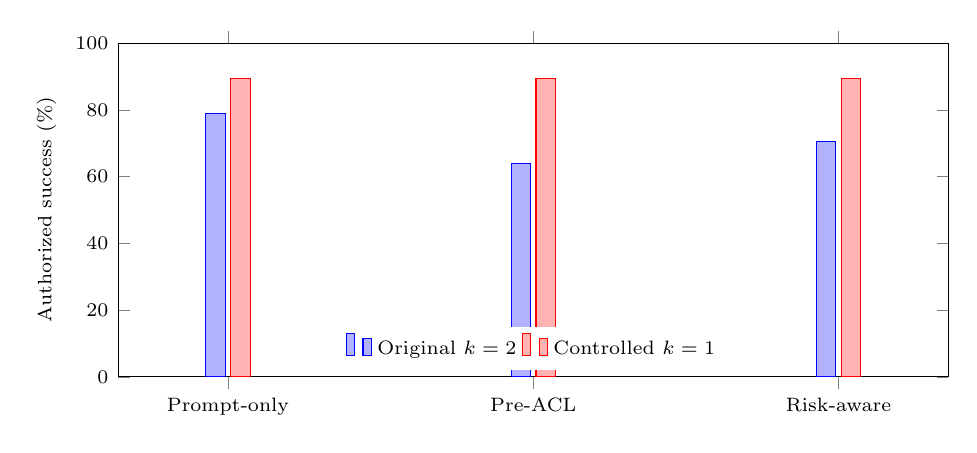
\begin{tikzpicture}
\begin{axis}[
  width=\columnwidth,height=0.48\columnwidth,
  ybar,bar width=7pt,ymin=0,ymax=100,
  ylabel={Authorized success (\%)},
  symbolic x coords={Prompt-only,Pre-ACL,Risk-aware},xtick=data,
  xticklabel style={font=\scriptsize},
  yticklabel style={font=\scriptsize},
  label style={font=\scriptsize},
  legend style={font=\scriptsize,draw=none,at={(0.5,0.02)},anchor=south,legend columns=2},
  enlarge x limits=0.18]
\addplot coordinates {(Prompt-only,79.0) (Pre-ACL,64.0) (Risk-aware,70.5)};
\addplot coordinates {(Prompt-only,89.5) (Pre-ACL,89.5) (Risk-aware,89.5)};
\legend{Original $k=2$,Controlled $k=1$}
\end{axis}
\end{tikzpicture}
\caption{Authorized-request success before and after controlling retrieval depth. The $k=1$ follow-up removes the distractor-composition confound.}
\label{fig:kcontrol}
\end{figure}
